\documentclass[11pt,a4paper]{scrartcl}
\typearea{12}
\usepackage{graphicx}
\usepackage{pstricks}
\usepackage{listings}
\lstset{language=python}
\pagestyle{headings}
\newcommand{\turtle}{\texttt{Turtle}\,}
\newcommand{\lnn}[1]{\textbf{line #1}\,}
\newcommand{\Lnn}[1]{\textbf{Line #1}\,}
\markright{Python turtle worksheet}
\begin{document}
\subsection*{Introduction}
Here is a simple turtle programme (\texttt{turtle\_doing\_nothing.py}):
\begin{lstlisting}[numbers=left]
from turtle import *

tom=Turtle()

tom.getscreen()._root.mainloop()
\end{lstlisting}
\Lnn{1} and \lnn{5} aren't worth spending much time on at first, the first
line imports the library of commands related to turtle, \lnn{5}
prevents the computer from closing the graphics window when the
programme has finished running; we won't include this line again,
though it is needed. \Lnn{3} is important, it tells the computer to
make an object, in this case a \turtle and call it \texttt{tom}, it
knows what a \turtle is from the library it imported in line 1; in the
instructions on what to do when making a \turtle the computer is told
to open a graphics window and to draw the turtle, a little arrow
shape.
\begin{center}
\fbox{

\includegraphics[width=10cm]{code/turtle_doing_nothing.eps}}
\end{center}

Here the turtle does something (\texttt{line.py}):
\begin{lstlisting}[numbers=left]
from turtle import *

tom=Turtle()

tom.forward(100)
\end{lstlisting}
The extra line, \lnn{5}, tells the turtle to move forward by 100 units,
this is an important piece of Python syntax, to tell an object to do
something you use a dot followed by the command, here it tells the
\turtle called \texttt{tom} to perform the command
\texttt{forward}. Of course, the command has to make sense for
whatever type of object it is dotted onto, but here it does,
\texttt{forward} is one of the defined commands for a \turtle object.
\begin{center}
\fbox{
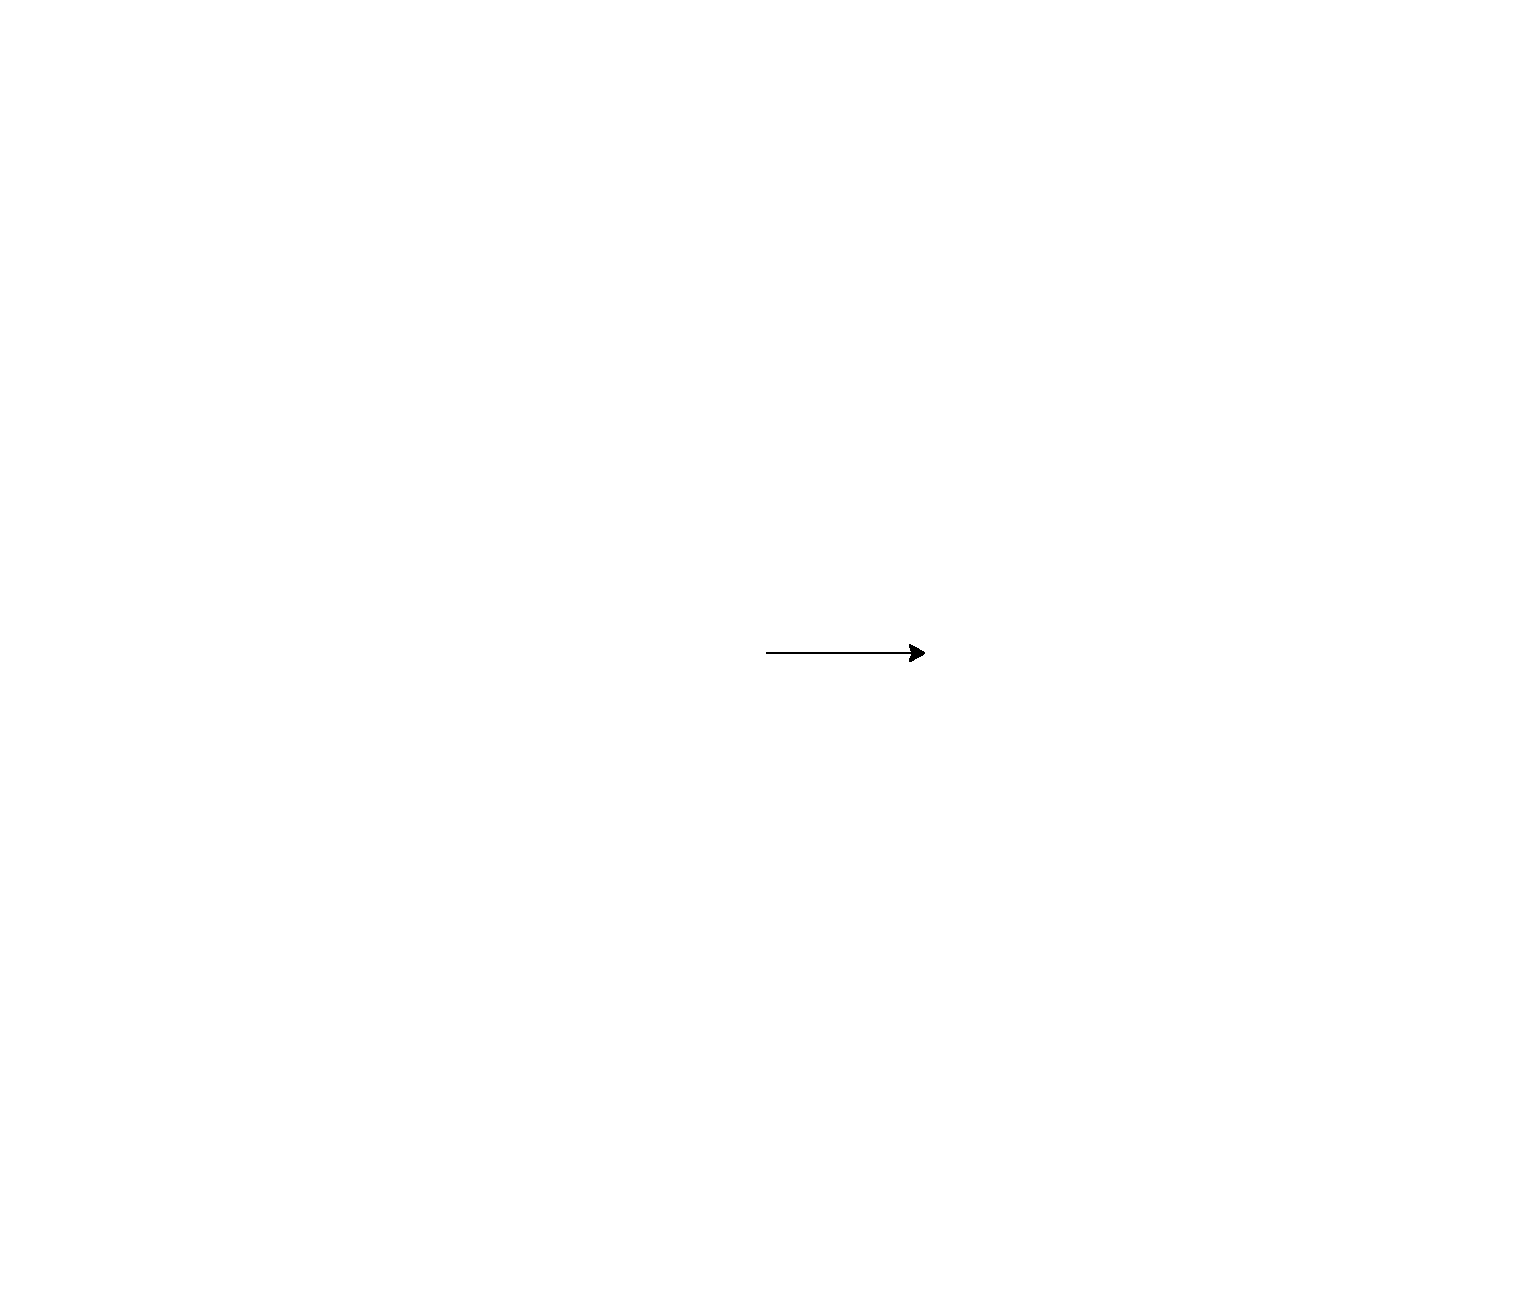
\includegraphics[width=10cm]{code/line.eps}}
\end{center}

\turtle objects have another command \texttt{right(90)} which turns the turtle by $90^\circ$. QUESTION: Can you write a programme to draw this:
\begin{center}
\fbox{
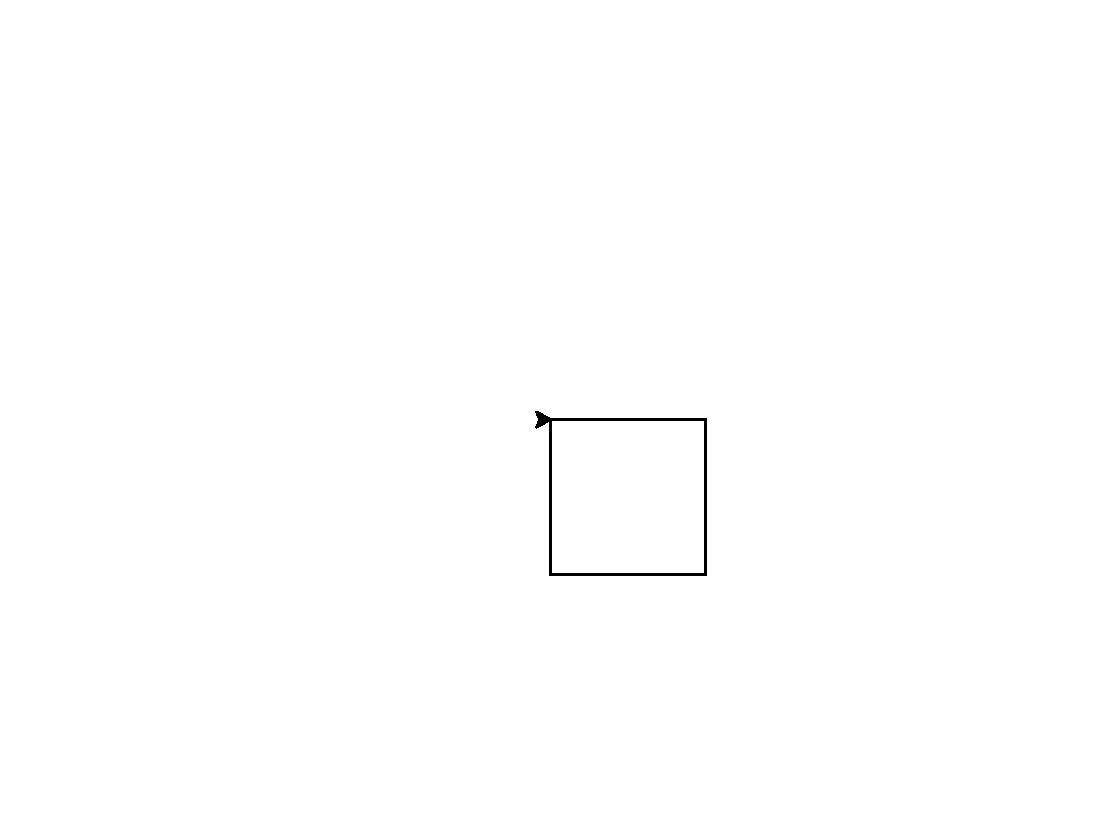
\includegraphics[width=10cm]{code/right_angle.eps}}
\end{center}
QUESTION: How about a square?
\begin{center}
\fbox{
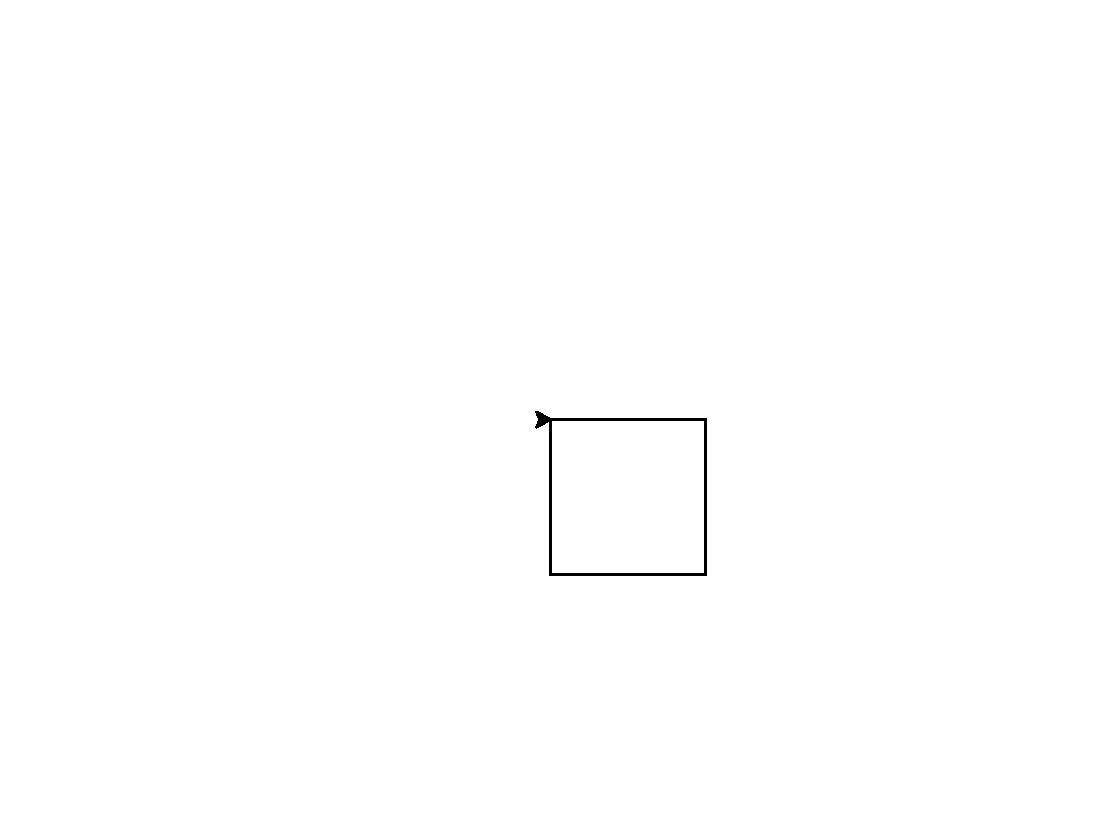
\includegraphics[width=10cm]{code/square.eps}}
\end{center}

Perhaps you programme to draw a square looked like this
\begin{lstlisting}[numbers=left]
from turtle import *

tom=Turtle()

tom.forward(100)
tom.right(90)
tom.forward(100)
tom.right(90)
tom.forward(100)
tom.right(90)
tom.forward(100)
tom.right(90)
\end{lstlisting}
There are two problems with this, most obviously it is boring writing
in the same two lines again and again; secondly, the programme is
inflexible and hard to read, we'll deal with the inflexible bit later,
but as for the hard to read, to know that it draws four lines and has
four corners you need to count the lines; it would be better if the
\lq{}fourness\rq{} was more apparent, as it is in this programme (\texttt{square\_loop}):
\begin{lstlisting}[numbers=left]
from turtle import *

tom=Turtle()

for i in range(0,4):
   tom.forward(100)
   tom.right(90)

\end{lstlisting}
The business part of this program is \textbf{line 5};
\texttt{range(0,4)} is the list of numbers \texttt{[0,1,2,3]}, so
starting at zero and ending one before four; the full command says
that \texttt{i} takes each value in this list in turn and then does
all the stuff belonging to the command. Here the command is a
\texttt{for}, a command that says \lq{}do everything that belongs to
the for once for every value the variable, in this case i, is
instructed to take\rq{}. In Python stuff belonging to a command is
indented, so that means it does \lnn{6} and \lnn{7} once for each item
in the list, that is four times. Of course, in this programme
\texttt{i} isn't used for anything except counting but it could be
(\texttt{spiral1.py}):
\begin{lstlisting}[numbers=left]
from turtle import *

tom=Turtle()

for i in range(0,8):
   tom.forward(100+10*i)
   tom.right(90)

\end{lstlisting}
giving
\begin{center}
\fbox{
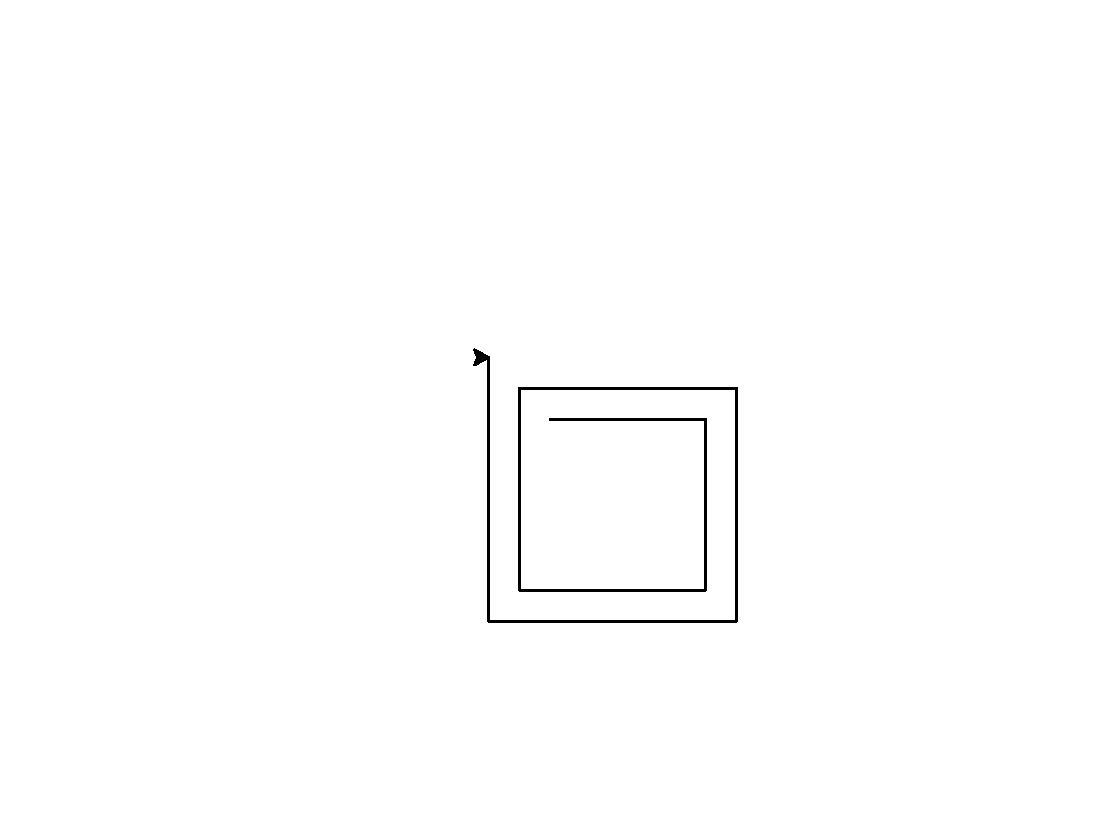
\includegraphics[width=10cm]{code/spiral1.eps}}
\end{center}
\texttt{i} is variable, it stores some data, in this case a number
which changes each time the programme goes around the \texttt{for}
loop. Once slightly confusing thing is \lq{}scoping\rq{}, which is
where the variable is defined; the \texttt{i} is only defined inside
the \texttt{for} loop, that is, it only exists while the programme is
executing \lnn{5} to \lnn{7}, but that's fine, that's where we use it.
QUESTION: Can you draw a triangular spiral like this:
\begin{center}
\fbox{

\includegraphics[width=10cm]{code/spiral2.eps}}
\end{center}

The list in the \texttt{for} loop doesn't have to be a \texttt{range},
in this example (\texttt{square\_color.py})
\begin{lstlisting}[numbers=left]
from turtle import *

tom=Turtle()

colors=['red','green','blue','yellow']

for color in colors:
    tom.pencolor(color)
    tom.forward(100)
    tom.right(90)
\end{lstlisting}
\texttt{colors} defined in \lnn{5} is a list of colours and the
variable in the \texttt{for} command takes each of these values in
turn. \texttt{pencolor} is another \turtle method, it changes the pen
colour so we get
\begin{center}
\fbox{
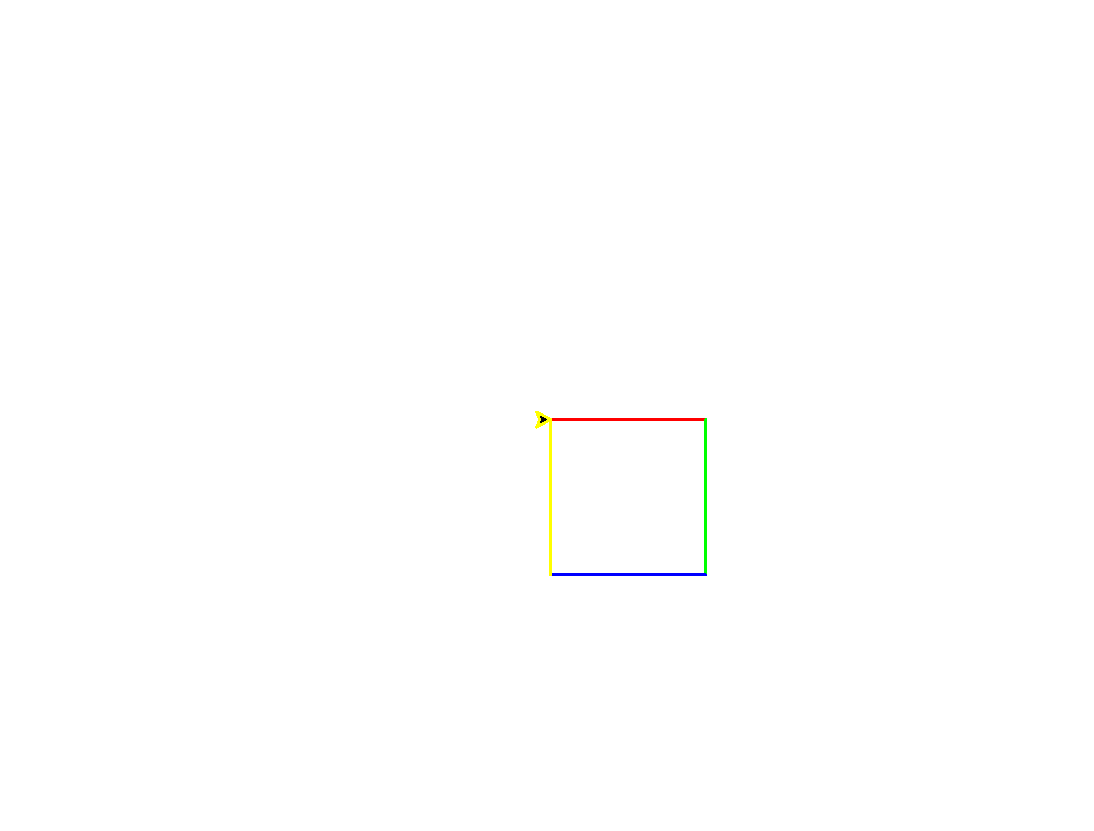
\includegraphics[width=10cm]{code/square_color.eps}}
\end{center}

In the colour example we use a variable \texttt{colors} to store a
list; here is an example where we use a variable to store an integer \texttt{n} which gives a number of sides.
\begin{lstlisting}[numbers=left]
from turtle import *

tom=Turtle()

n=8

for i in range(0,n):
    tom.forward(100)
    tom.right(360.0/n)

\end{lstlisting}
This is useful because we need the number of sides twice, once in
\lnn{7} where it gives the number of sides, and the second time in
\lnn{9} where it is used to calculate the turning angle. Obviously it
would be possible to write the number in those two places, but that
would be a very bad programming style because it would mean changing
it in those two places if you wanted to change the number of sides to
the polygon. It would be easy to get this wrong, maybe not for only
two places, but in a more complex programme there may be many places a
value needs to be changed, leading to errors. Furthermore, keeping
\texttt{n} seperate makes the programme easier to understand.

Now imagine you wanted to draw this:
\begin{center}
\fbox{
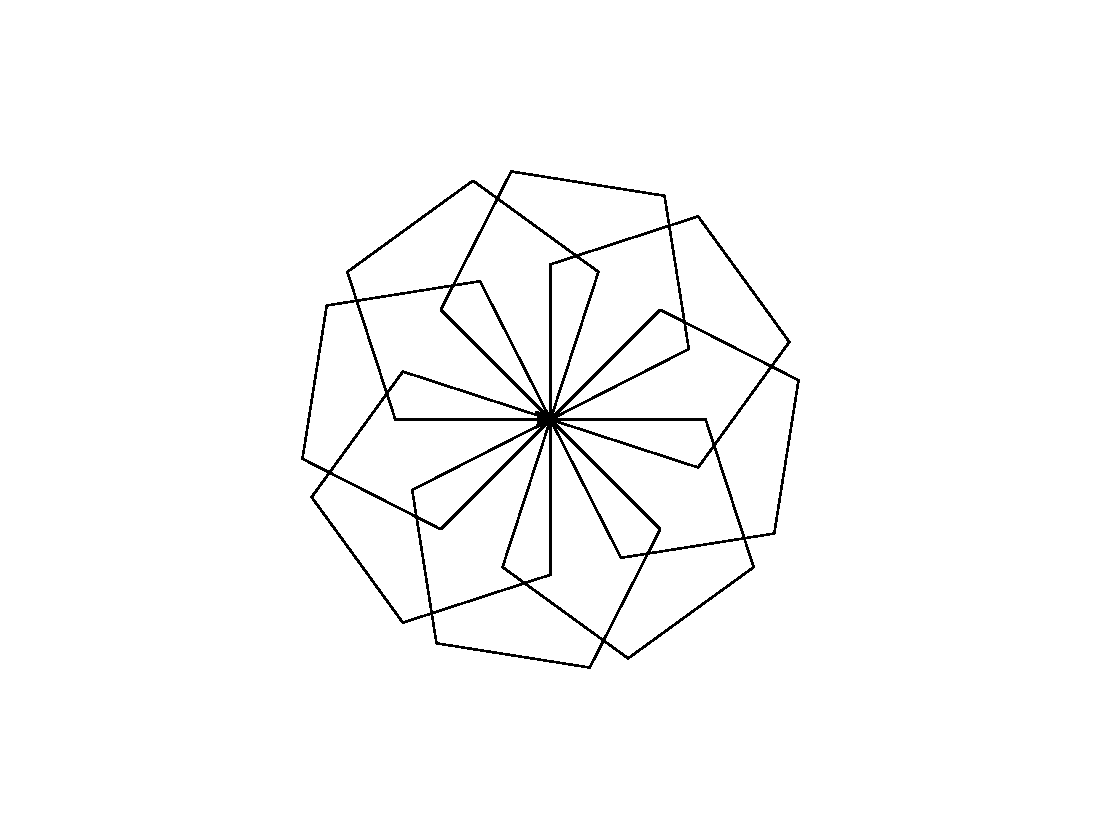
\includegraphics[width=10cm]{code/many_polygons.eps}}
\end{center}
This is made of eight pentagons with an eighth of a full turn between
each one; this can be made using the programme:
\begin{lstlisting}[numbers=left]
from turtle import *

tom=Turtle()

repeats=8
polygon_sides=5

for i in range(0,repeats):
   for j in range(0,polygon_sides):
       tom.forward(100)
       tom.right(360.0/polygon_sides)
   tom.right(360/repeats)
\end{lstlisting}
So this programme has two \texttt{for} loops, the \texttt{j} loop from
\lnn{8} to \lnn{10} draws the pentagons, the \texttt{i} loop repeats
that eight times and rotates between pentagon. Notice the two loops
need different variables, \texttt{i} and \texttt{j}, and you can tell
what belongs to which loop by the indent, \lnn{9} and \lnn{10} belong
to the \texttt{j} loop so these command are run $40=8\times 5$ times
whereas \lnn{9} and \lnn{11} are only run eight times.

This programme works, but it fails our readibility and adaptability
test; to work out what it does you need to figure your way through the
double loop and if you wanted to draw another pentagon later you would
have to cut and paste the lines you already had. A much better
programme would use a function (\texttt{many\_polygons.py}):
\begin{lstlisting}[numbers=left]
from turtle import *

def polygon(n):

    for i in range(0,n):
        tom.forward(100)
        tom.right(360.0/n)

tom=Turtle()

repeats=8
polygon_sides=5

for i in range(0,repeats):
    polygon(5)
    tom.right(360.0/repeats)
\end{lstlisting}
Now in \lnn{3} to \lnn{7} we have defined a \texttt{function}, the
command \texttt{def} announces in \lnn{3} that a function definition
is on the way, all the indented lines are the definition. The function
is named \texttt{polygon}; the brackets after the function name are to
give the arguements, values that are sent to the function, in this
case the function has one arguement which will give the number of
sides of the polygon. Now we have a new command, \texttt{polygon(n)},
whenever the command is given, the programme goes up to the function
and runs the code belonging to the function, this happens in \lnn{17}.

QUESTION: can you guess how this was drawn:
\begin{center}
\fbox{
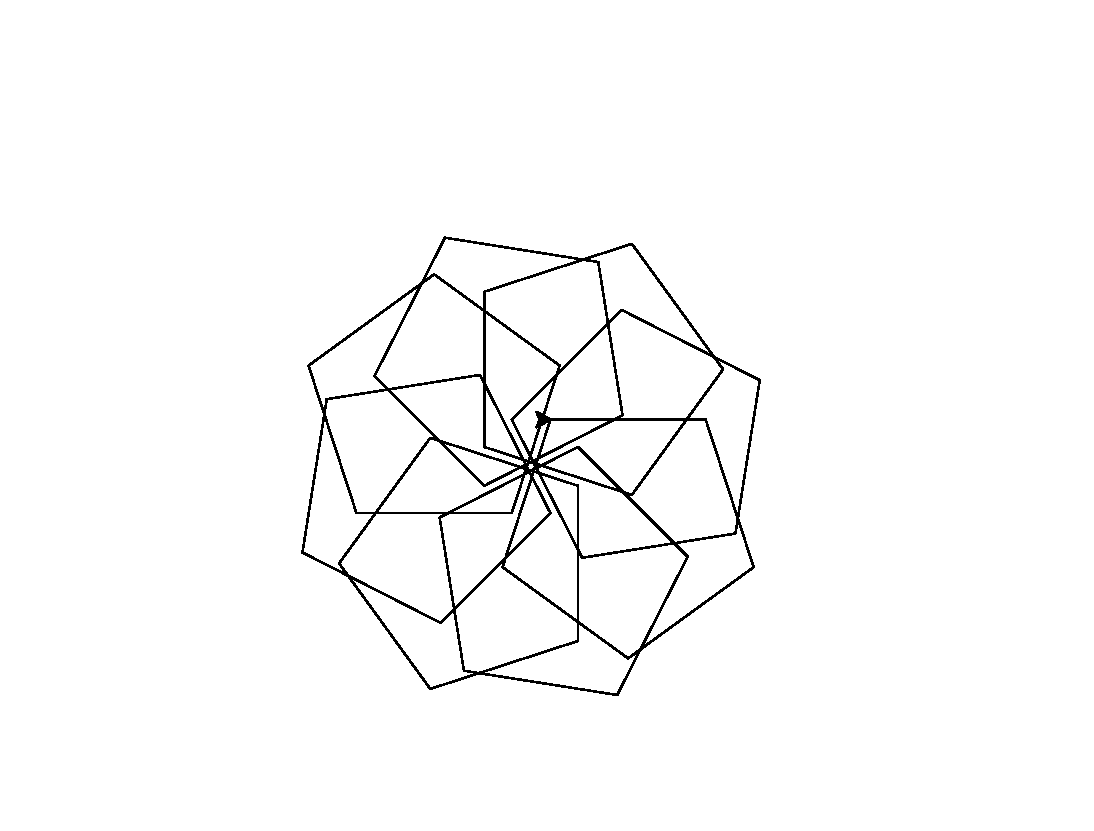
\includegraphics[width=10cm]{code/many_polygons_extra.eps}}
\end{center}
The \turtle commands \texttt{penup()} and \texttt{pendown()} lift and
drop the turtle's pen, when the pen is up the turtle moves without
leaving a line.


\end{document}

